\clearpage
\section{O1: Additional analysis}
\label{app:o1-additional}
\begin{authorcontribution}{authorSowmya}
\renewcommand{\arraystretch}{1.2}
\subsection{O1: Data cleaning rules and log}
\label{app:o1-cleaning}
Rules in \texttt{clean()} drop only structurally empty rows, flag others for sensitivity runs, or aggregate; no observed value is overwritten.

\textbf{C1 Schema:} coerce numeric fields; drop rows missing a key. \textbf{C2 Names:} trim spaces; the AirAsia India $\to$ AIX Connect rebrand (January 2024) is kept as reported. \textbf{C3 Scope:} scheduled domestic, January 2015--July 2026. \textbf{C4 Duplicates:} sum rows for the same airline-month. \textbf{C5 Structural zeros:} drop rows with passengers $\leq0$. \textbf{C6 Consistency:} flag seat-km $\leq0$ with passengers $>0$, or passenger-km above seat-km; keep. \textbf{C7 Outliers:} flag $|\Delta\ln q|>0.7$; explained if in the COVID window or a market-wide move above 0.5 log points, an entry or exit ramp, or the merger month; otherwise immaterial (share $<1\%$) or material (checked by hand); never deleted, tested by dropping. \textbf{C8 Completeness:} list missing months and runs inside operating spells; April 2020 is left empty, COVID suspensions are real zeros, and material gaps are interpolated in a sensitivity run only. \textbf{C9 Share closure:} recompute shares from passengers; shares sum to 100 each month.

\begin{minipage}{\linewidth}
\captionsetup{font={small,color=authorSowmya},labelfont=bf,justification=raggedright,singlelinecheck=false,hypcap=false}
\captionof{table}{O1: Cleaning log, what each rule found and did.}
\label{tab:o1-cleaning}
\centering
{\footnotesize\setstretch{1.0}\setlength{\tabcolsep}{4pt}
\begin{tabularx}{\linewidth}{|>{\raggedright\arraybackslash}p{0.05\linewidth}|>{\raggedright\arraybackslash}X|>{\raggedright\arraybackslash}p{0.27\linewidth}|}
\hline
\textbf{Rule} & \textbf{Finding} & \textbf{Action} \\
\hline
C1 & 0 rows with a missing key field & None needed \\
\hline
C3 & 1,773 rows outside scheduled domestic service; none after July 2026 & Excluded \\
\hline
C4 & 0 duplicate airline-months & None needed \\
\hline
C5 & 132 scheduled-domestic rows with zero passengers & Dropped (not flying) \\
\hline
C6 & 2 rows with passengers $>0$ but seat-km $=0$ (Air Odisha, Sep 2018; Air Deccan, Mar 2020); no row with passenger-km $>$ seat-km & Flagged, kept \\
\hline
C7 & 92 outlier flags: 45 COVID or market-wide, 23 entry/exit ramp, 1 merger month, 23 unexplained but immaterial ($<1\%$ share), 0 material & Explained flags kept; immaterial ones tested by dropping \\
\hline
C8 & April 2020 missing for every airline; 12 runs missing inside operating spells, of which 2 are material: AirAsia India January--December 2017 (bracketing share 3.6\%) and Go First May 2020 (lockdown suspension) & 2017 gap interpolated in the sensitivity run only; Go First not imputed \\
\hline
C9 & Shares sum to 100 in all 138 months & Passes \\
\hline
\end{tabularx}\par}
\vspace{4pt}
{\footnotesize\setstretch{1.0}\raggedright\textit{Source:} \texttt{carrier\_monthly.csv} (SHA-256 \texttt{30412b65\ldots}); rules implemented in \texttt{o1\_analysis.py}.\par}
\end{minipage}

\clearpage
\subsection{O1: Robustness of the steps}
\label{app:o1-robust}
The Ownership-HHI steps do not depend on the lag choice or the COVID treatment: no coefficient moves by more than 19 points and every $t$-statistic stays at 2.2 or above (Table~\ref{tab:o1-robust}). Interpolating AirAsia India's 2017 raises the Jet step by 59 points and the others by at most 20. Re-dating the Jet and Go First steps to the drifts gives steps of 396, 933, 696 and 186 points (sum 2,211, $R^2=0.985$); the Brand-HHI sum is 1,801 and the MHHI sum 2,162, all steps significant at 1\%.

\begin{minipage}{\linewidth}
\captionsetup{font={small,color=authorSowmya},labelfont=bf,justification=raggedright,singlelinecheck=false,hypcap=false}
\captionof{table}{O1: Robustness of the Ownership-HHI steps (coefficient, $t$-statistic).}
\label{tab:o1-robust}
\centering
{\small\setstretch{1.1}\setlength{\tabcolsep}{5pt}
\begin{tabular}{|l|r|r|r|r|}
\hline
\textbf{Specification} & \textbf{Jet exit} & \textbf{Tata} & \textbf{Go First} & \textbf{Mergers} \\
\hline
Baseline (Newey--West 12 lags) & 312 (3.9) & 900 (10.8) & 640 (11.4) & 137 (2.5) \\
\hline
Newey--West 6 lags & 312 (3.8) & 900 (9.8) & 640 (10.4) & 137 (2.2) \\
\hline
Newey--West 18 lags & 312 (4.6) & 900 (12.1) & 640 (12.0) & 137 (2.8) \\
\hline
COVID months dropped & 330 (4.6) & 899 (10.6) & 656 (12.0) & 136 (2.5) \\
\hline
AirAsia India 2017 interpolated & 371 (4.0) & 920 (10.0) & 652 (10.6) & 148 (2.6) \\
\hline
\end{tabular}\par}
\end{minipage}
\vspace{0.8em}
\textbf{O1 reproduction.} The script \texttt{o1\_analysis.py} recomputes every O1 number from the passenger file \texttt{carrier\_monthly.csv}, covering cleaning, indices, drift detection, regressions and robustness checks. The script \texttt{plot\_index\_over\_\allowbreak months.py} reproduces Figure~\ref{fig:o1-its}.

\clearpage
\subsection{O1: Concentration figure}
\begin{minipage}{\linewidth}
\centering
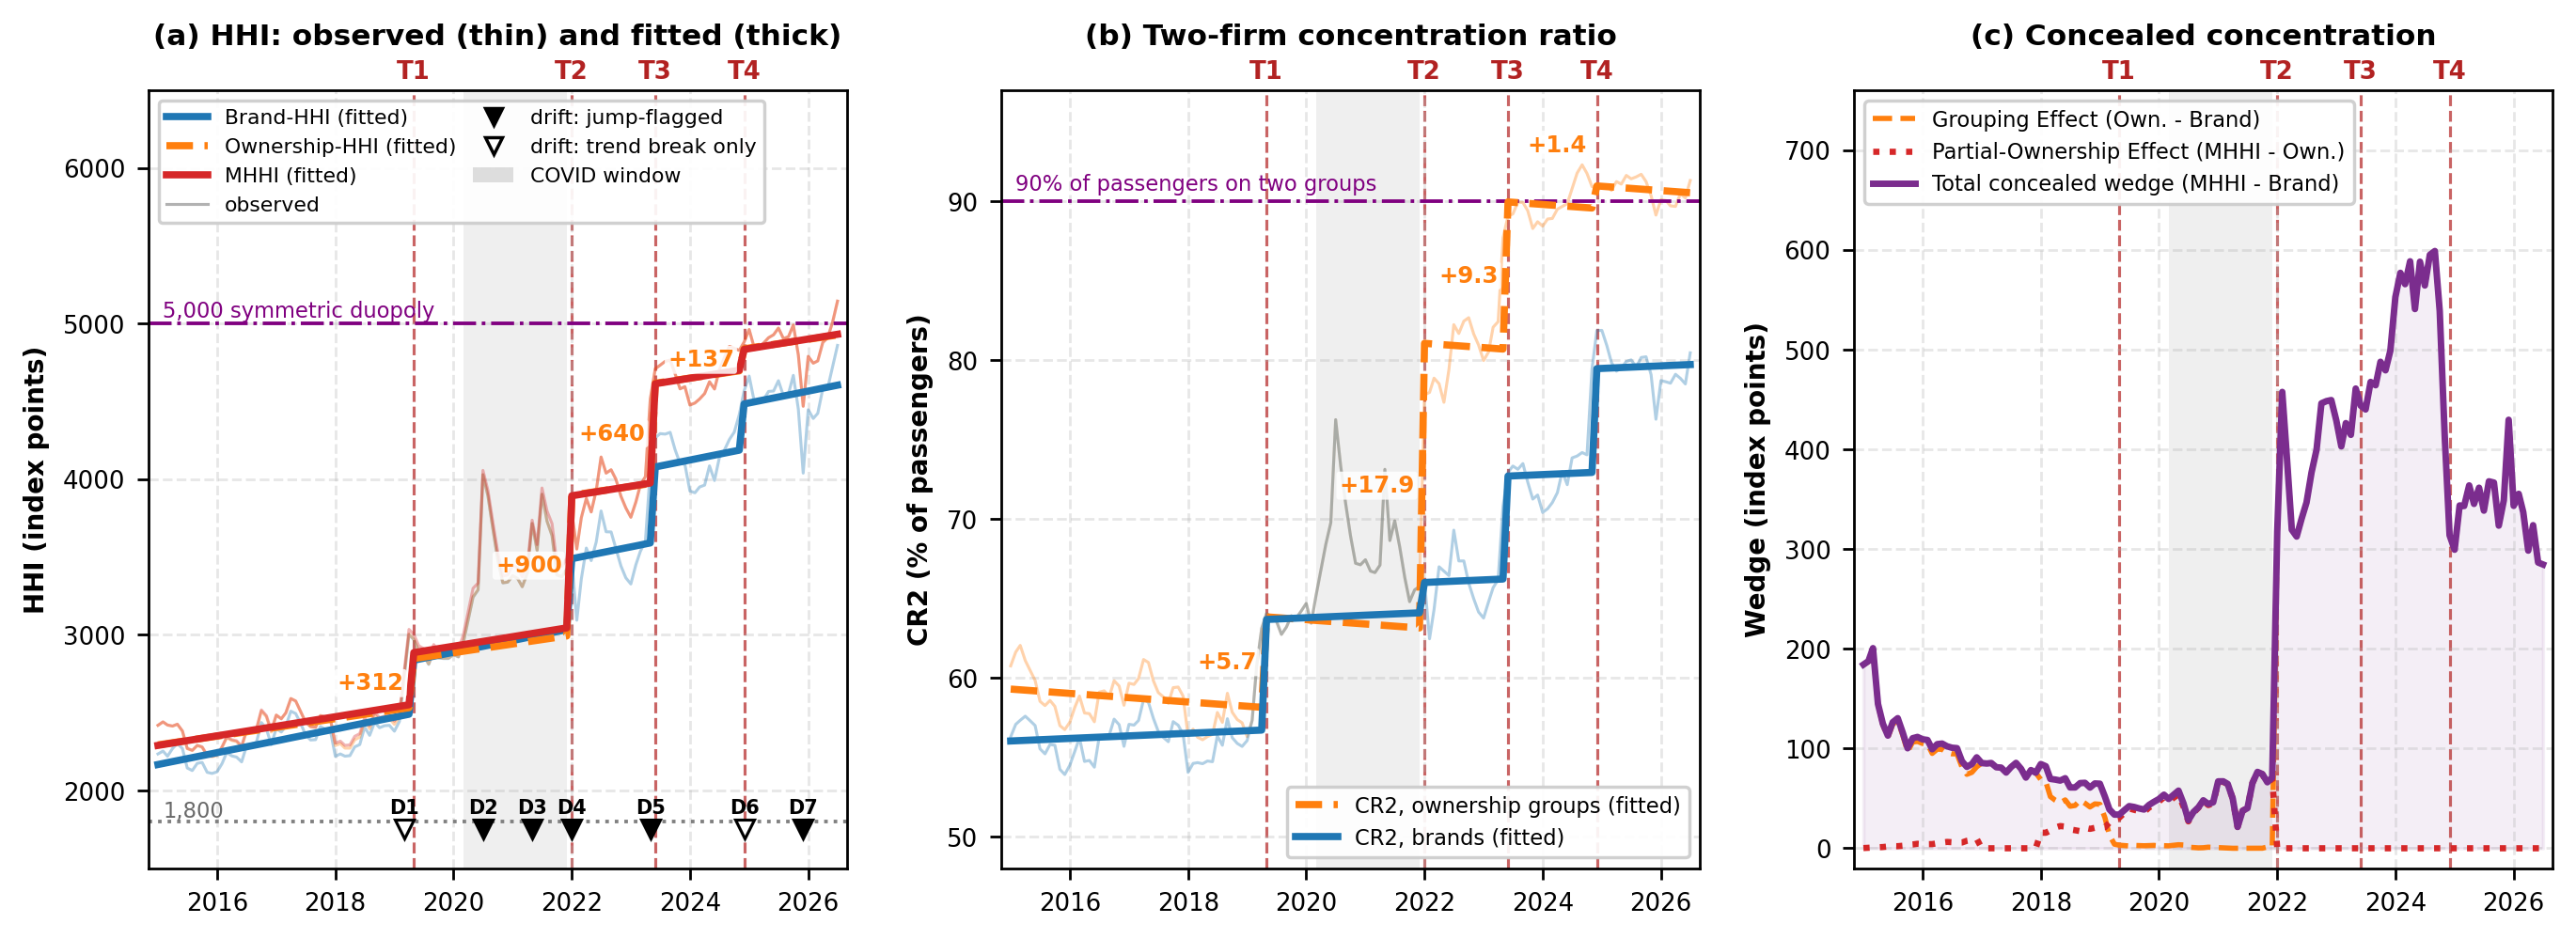
\includegraphics[width=\linewidth]{figures/o1_hhi.png}
\captionsetup{font={small,color=authorSowmya},labelfont=bf,hypcap=false}
\captionof{figure}{O1: Interrupted time-series view of national concentration, January 2015--July 2026.}
\label{fig:o1-its}
\vspace{2pt}
\par\footnotesize\setstretch{1.1}
\textit{Note:} (a) Brand-, Ownership- and MHHI: observed (thin) and fitted (thick) values from Equation~O1.2, keeping the trend and the four event steps, with COVID and month-of-year terms netted out; figures beside each step are Ownership-HHI steps in points. (b) CR2 with its steps in percentage points. (c) Grouping Effect, Partial-Ownership Effect and their sum, the total concealed wedge. T1--T4: Jet exit, Tata acquisition, Go First exit, legal mergers. D1--D7: drift points (filled markers flagged by the jump detector). Grey band: COVID window.\par
\textit{Source:} DGCA monthly traffic via \href{https://github.com/mkubicek/india-aviation-stats/tree/16770ac59dae61ce7b80fd8bd67dd7f4cef280a6}{Kubicek (2026)}; authors' calculations.
\end{minipage}
\end{authorcontribution}
